\section{Projekt interfejsu użytkownika}
W niniejszym podrodziale został zaprezentowany projekt interfejsu użytkownika
projektowanej aplikacji. Kolejne okna aplikacji prezentowane są w takiej samej
kolejności jak przypadki użycia opisane w rozdziale \ref{chap:przypadki-uzycia}.

\subsection{Zarządzanie systemem}
\begin{figure}[!htb]
  \begin{center}
    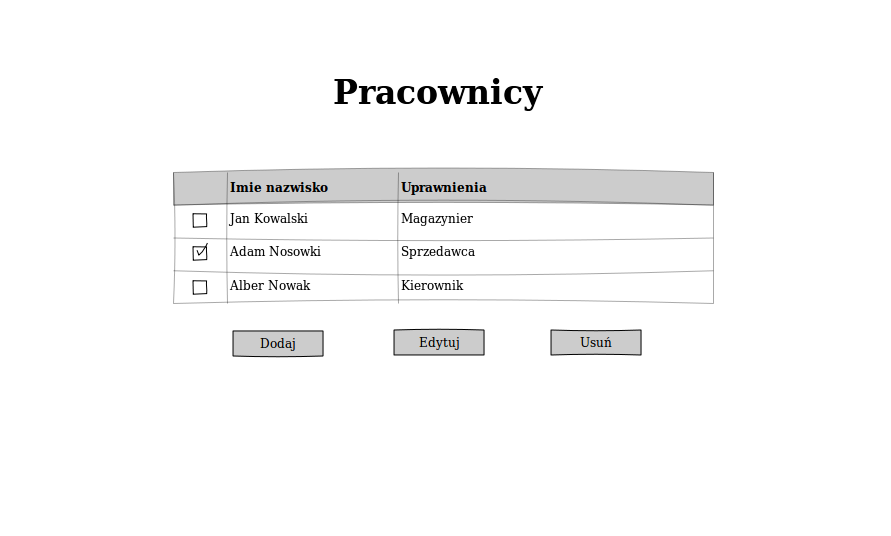
\includegraphics[scale=0.45]{../img/interfejs/zarzadzanie-pracownikami.png}
  \end{center}
  \caption{Okno zarządzania pracownikami}
\end{figure}
\FloatBarrier

\begin{figure}[!htb]
  \begin{center}
    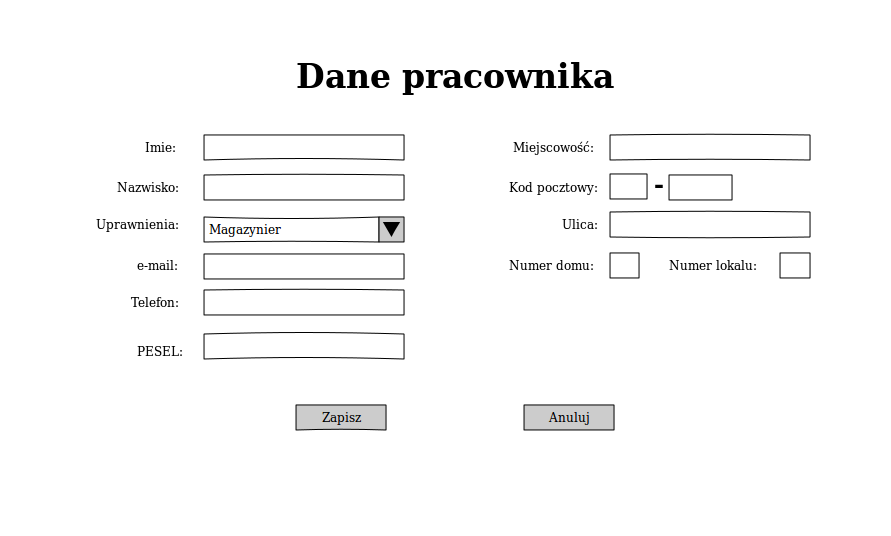
\includegraphics[scale=0.45]{../img/interfejs/utworzenie-pracownika.png}
  \end{center}
  \caption{Okno dodania nowego pracownika}
\end{figure}
\FloatBarrier

\begin{figure}[!htb]
  \begin{center}
    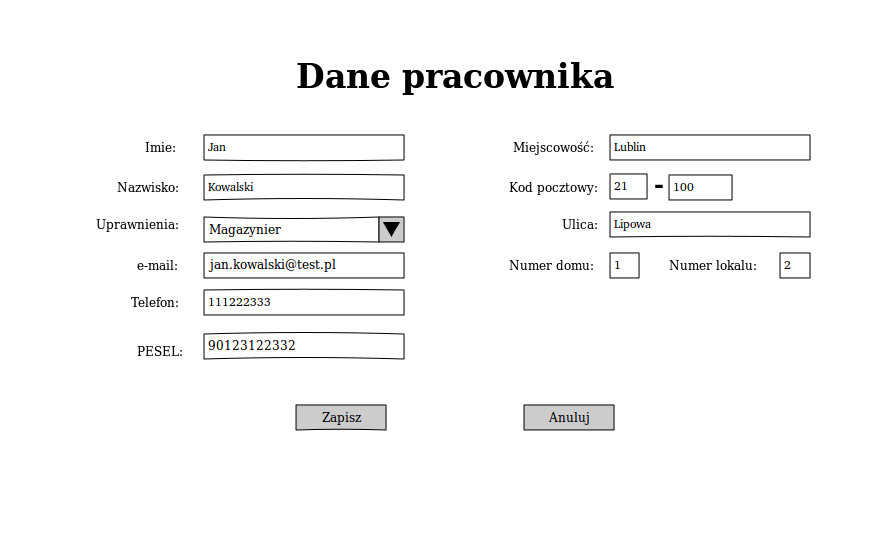
\includegraphics[scale=0.45]{../img/interfejs/edycja-pracownika.png}
  \end{center}
  \caption{Okno edycji danych pracownika}
\end{figure}
\FloatBarrier

\begin{figure}[!htb]
  \begin{center}
    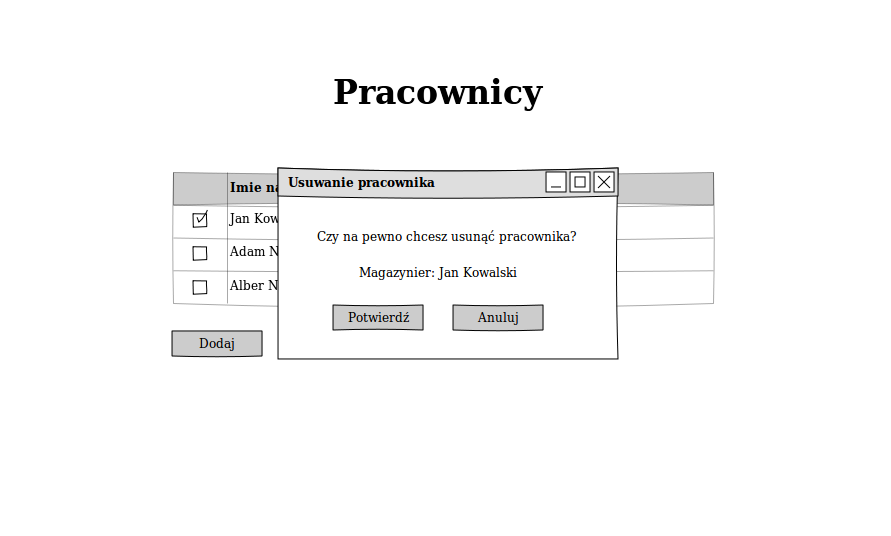
\includegraphics[scale=0.45]{../img/interfejs/usuniecie-pracownika.png}
  \end{center}
  \caption{Okno usunięcia danych pracownika}
\end{figure}
\FloatBarrier

\begin{figure}[!htb]
  \begin{center}
    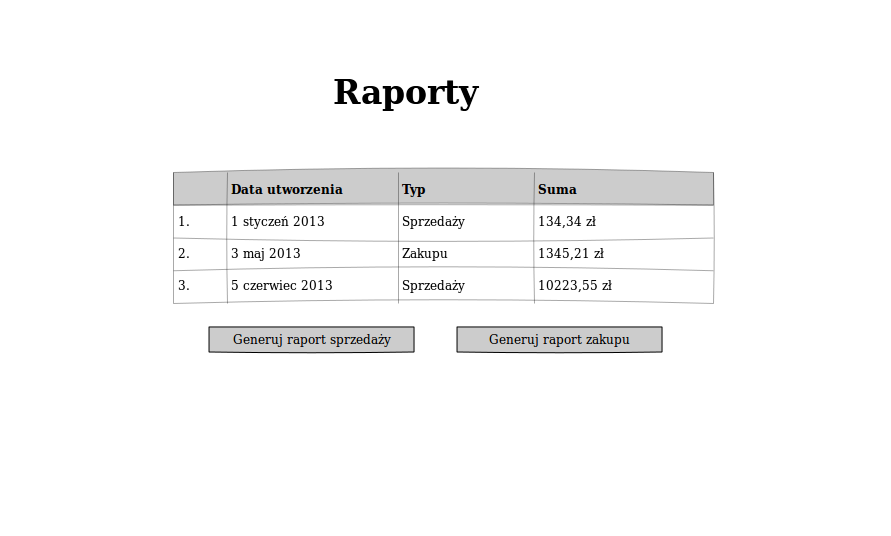
\includegraphics[scale=0.45]{../img/interfejs/zarzadzanie-raportami.png}
  \end{center}
  \caption{Okno zarządzania raportami}
\end{figure}
\FloatBarrier

\begin{figure}[!htb]
  \begin{center}
    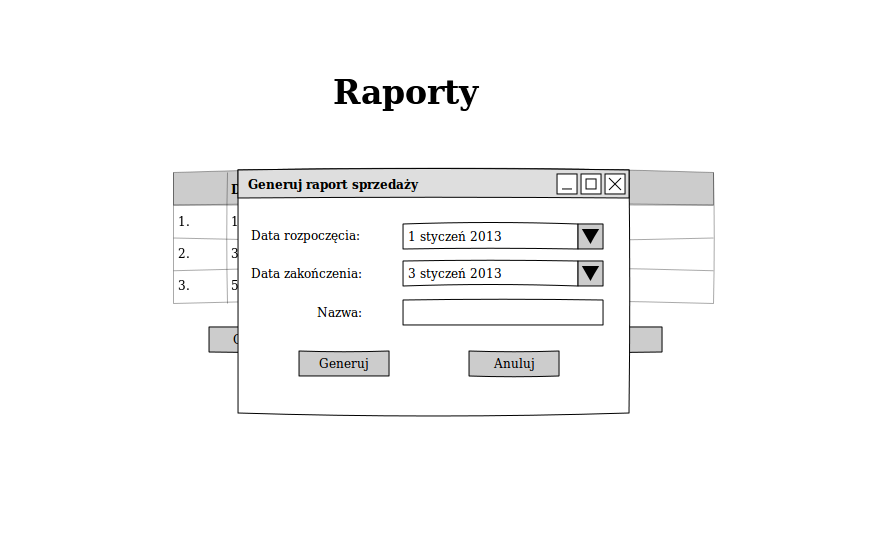
\includegraphics[scale=0.45]{../img/interfejs/generowanie-raportu-sprzedazy.png}
  \end{center}
  \caption{Okno generowania raportu danych wydania towarów}
\end{figure}
\FloatBarrier

\begin{figure}[!htb]
  \begin{center}
    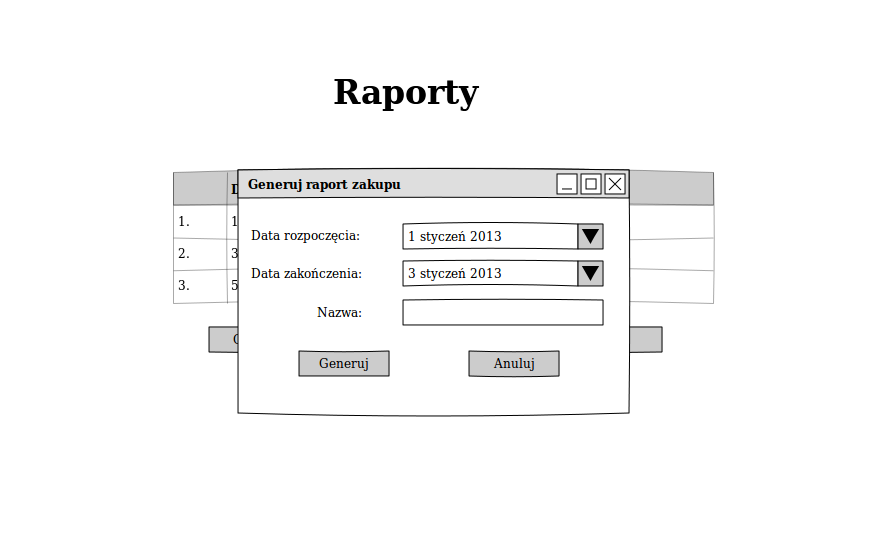
\includegraphics[scale=0.45]{../img/interfejs/generowanie-raportu-zakupow.png}
  \end{center}
  \caption{Okno generowania raportu przyjęcia towarów}
\end{figure}
\FloatBarrier

\subsection{Obsługa kontrahentów}

\begin{figure}[!htb]
  \begin{center}
    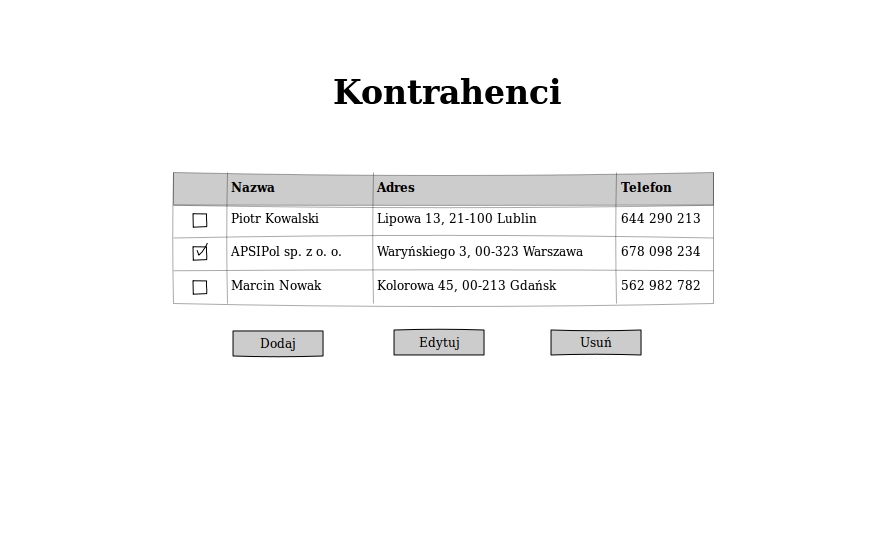
\includegraphics[scale=0.45]{../img/interfejs/zarzadzanie-kontrahentami.png}
  \end{center}
  \caption{Okno zarządzania danymi kontrahentów}
\end{figure}
\FloatBarrier

\begin{figure}[!htb]
  \begin{center}
    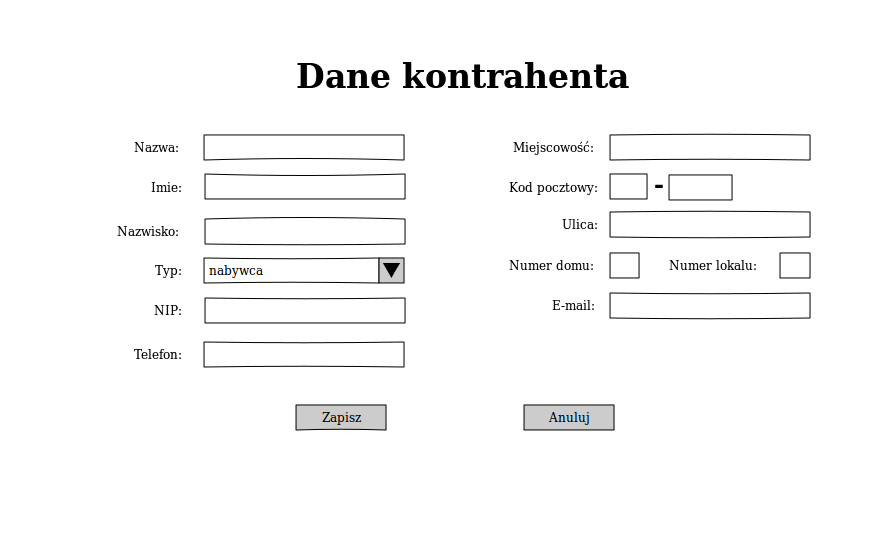
\includegraphics[scale=0.45]{../img/interfejs/utworzenie-kontrahenta.png}
  \end{center}
  \caption{Okno tworzenia nowego kontrahenta}
\end{figure}
\FloatBarrier

\begin{figure}[!htb]
  \begin{center}
    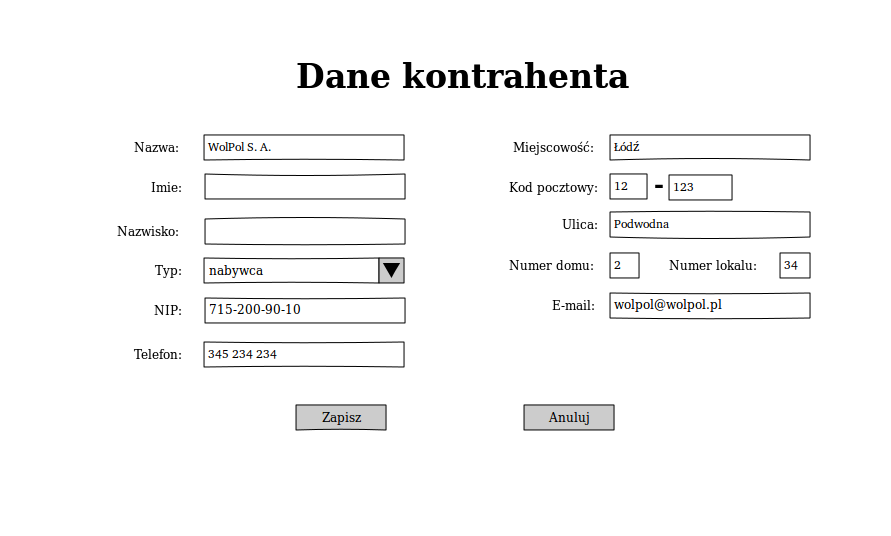
\includegraphics[scale=0.45]{../img/interfejs/edycja-kontrahenta.png}
  \end{center}
  \caption{Okno edycji danych kontrahenta}
\end{figure}
\FloatBarrier

\begin{figure}[!htb]
  \begin{center}
    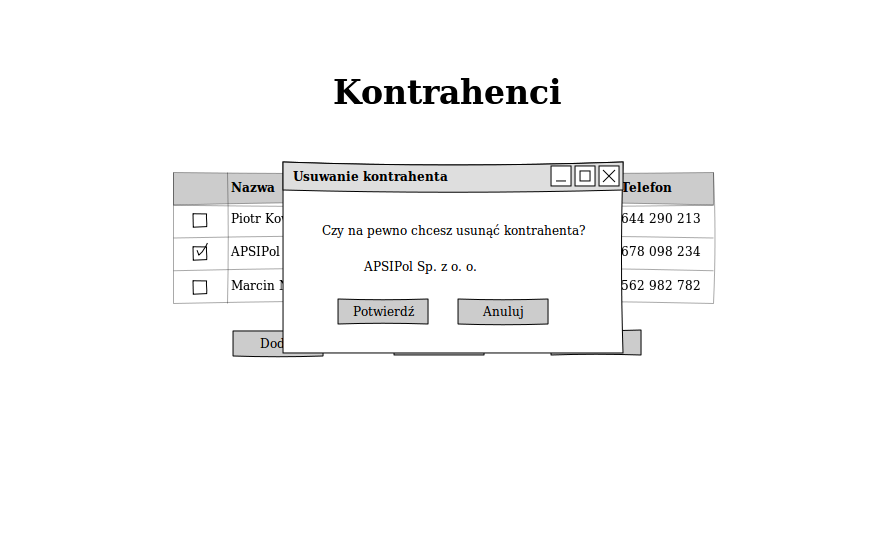
\includegraphics[scale=0.45]{../img/interfejs/usuwanie-danych-kontrahenta.png}
  \end{center}
  \caption{Okno usunięcia danych kontrahenta}
\end{figure}
\FloatBarrier

\subsection{Sprzedaż}

\begin{figure}[!htb]
  \begin{center}
    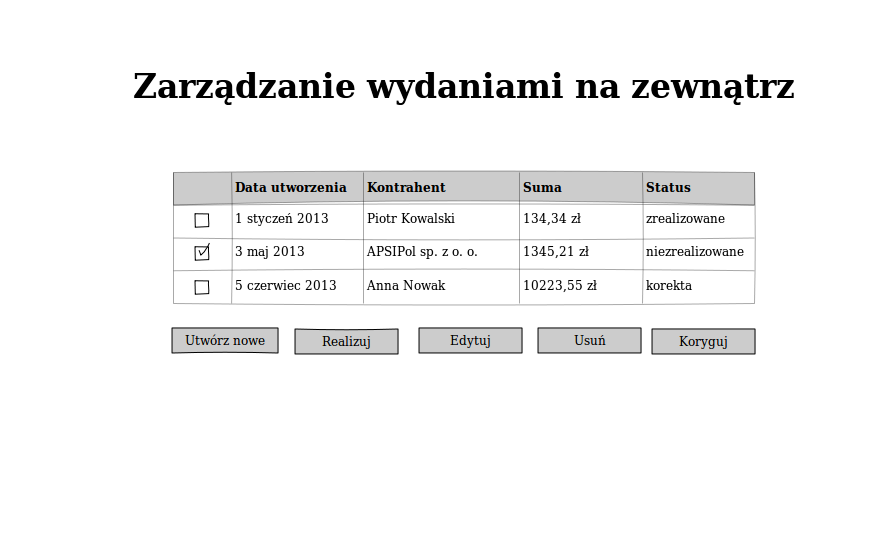
\includegraphics[scale=0.45]{../img/interfejs/zarzadzanie-dokumentami-WZ.png}
  \end{center}
  \caption{Okno zarządzania dokumentami wydania na zewnątrz}
\end{figure}
\FloatBarrier

\begin{figure}[!htb]
  \begin{center}
    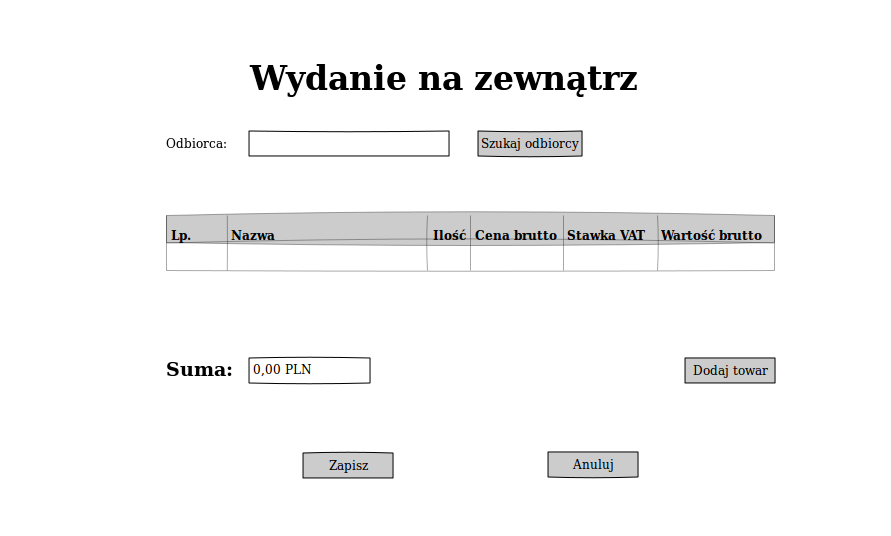
\includegraphics[scale=0.45]{../img/interfejs/utworzenie-wydania-na-zewnatrz.png}
  \end{center}
  \caption{Okno utworzenia dokumentu wydania na zewnątrz}
\end{figure}
\FloatBarrier

\begin{figure}[!htb]
  \begin{center}
    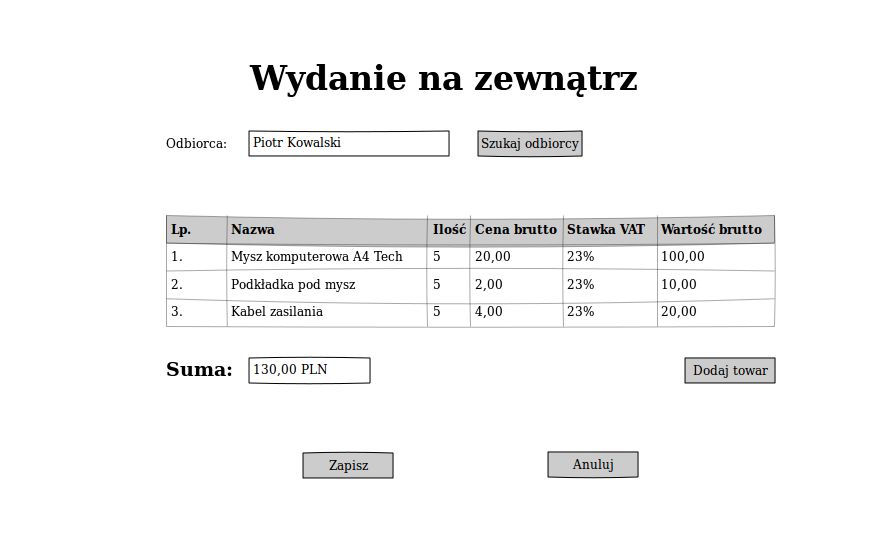
\includegraphics[scale=0.45]{../img/interfejs/edycja-wydania-na-zewnatrz.png}
  \end{center}
  \caption{Okno edycji wydania na zewnątrz}
\end{figure}
\FloatBarrier

\begin{figure}[!htb]
  \begin{center}
    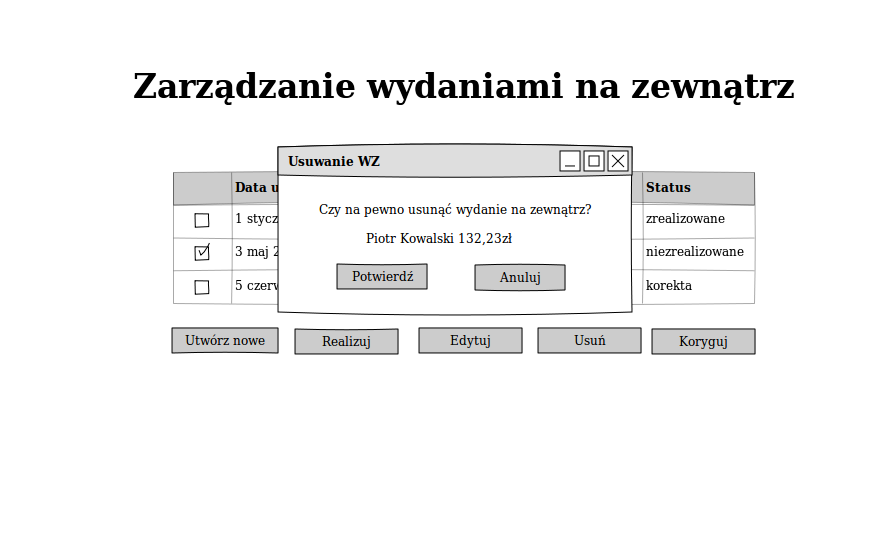
\includegraphics[scale=0.45]{../img/interfejs/usuniecie-wydania-na-zewnatrz.png}
  \end{center}
  \caption{Okno usunięcia dokumentu wydania na zewnątrz}
\end{figure}
\FloatBarrier

\begin{figure}[!htb]
  \begin{center}
    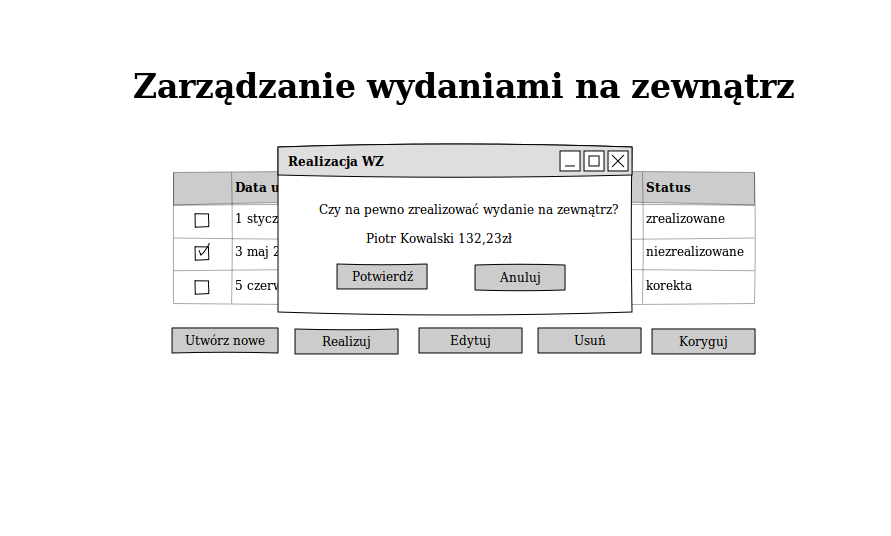
\includegraphics[scale=0.45]{../img/interfejs/realizacja-wydania-na-zewnatrz.png}
  \end{center}
  \caption{Okno realizacji wydania na zewnątrz}
\end{figure}
\FloatBarrier

\begin{figure}[!htb]
  \begin{center}
    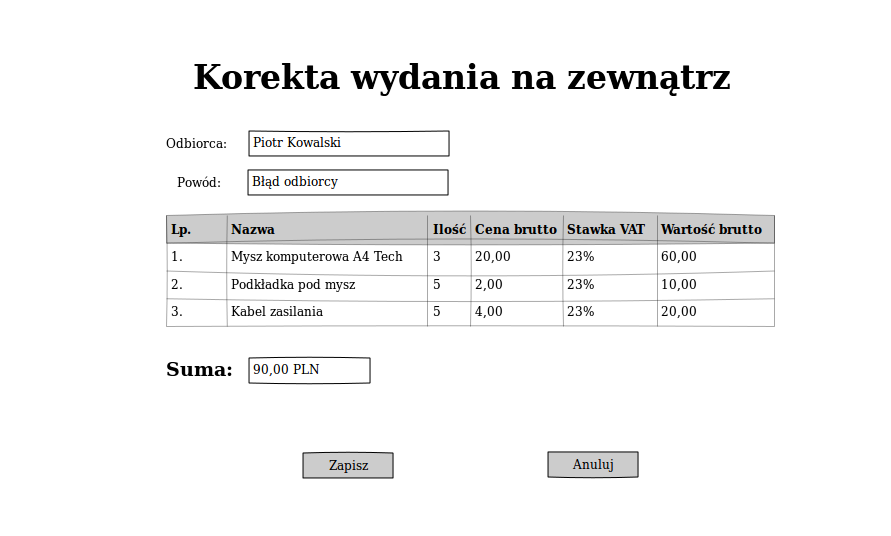
\includegraphics[scale=0.45]{../img/interfejs/korekta-wydania-na-zewnatrz.png}
  \end{center}
  \caption{Okno korekty wydania na zewnątrz}
\end{figure}
\FloatBarrier

\subsection{Zarządzanie towarami}

\begin{figure}[!htb]
  \begin{center}
    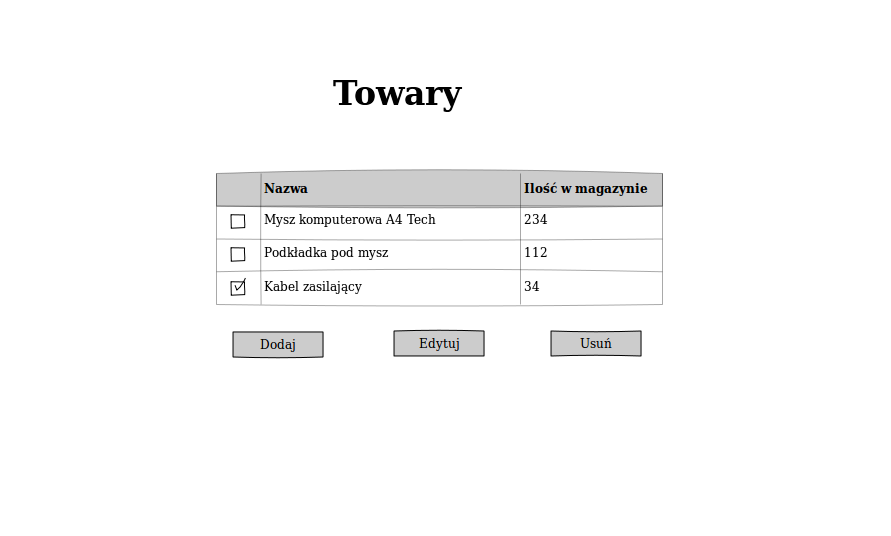
\includegraphics[scale=0.45]{../img/interfejs/zarzadzanie-towarami.png}
  \end{center}
  \caption{Okno zarządzania danymi towarów}
\end{figure}
\FloatBarrier

\begin{figure}[!htb]
  \begin{center}
    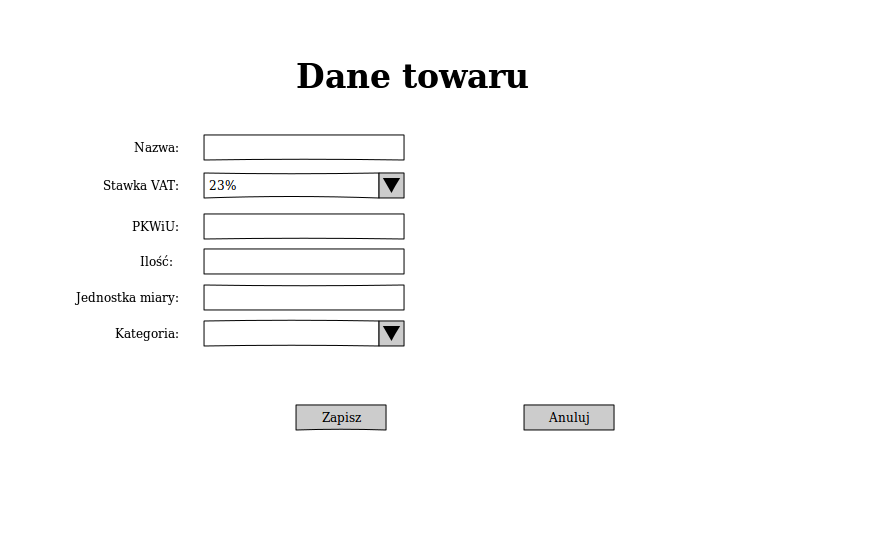
\includegraphics[scale=0.45]{../img/interfejs/dodanie-danych-towaru.png}
  \end{center}
  \caption{Okno dodawania danych towaru}
\end{figure}
\FloatBarrier

\begin{figure}[!htb]
  \begin{center}
    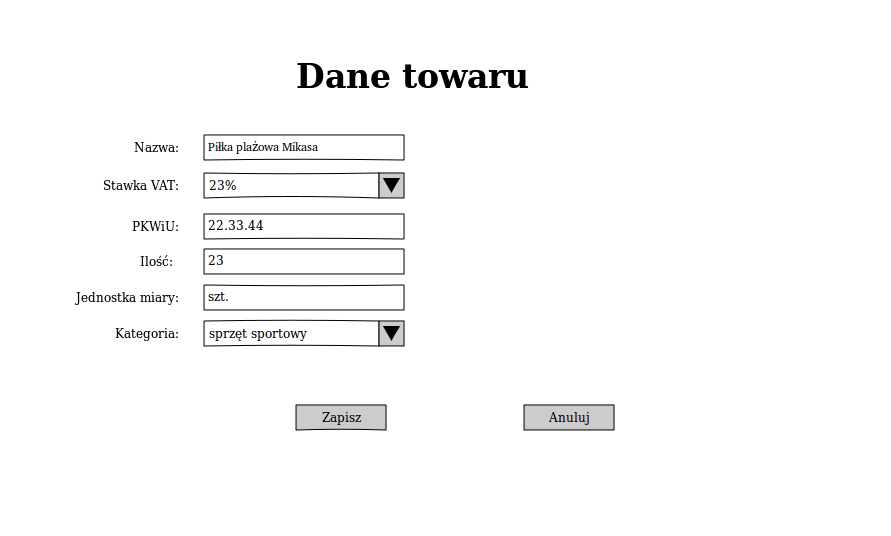
\includegraphics[scale=0.45]{../img/interfejs/edycja-danych-towaru.png}
  \end{center}
  \caption{Okno edycji opisu towaru}
\end{figure}
\FloatBarrier

\begin{figure}[!htb]
  \begin{center}
    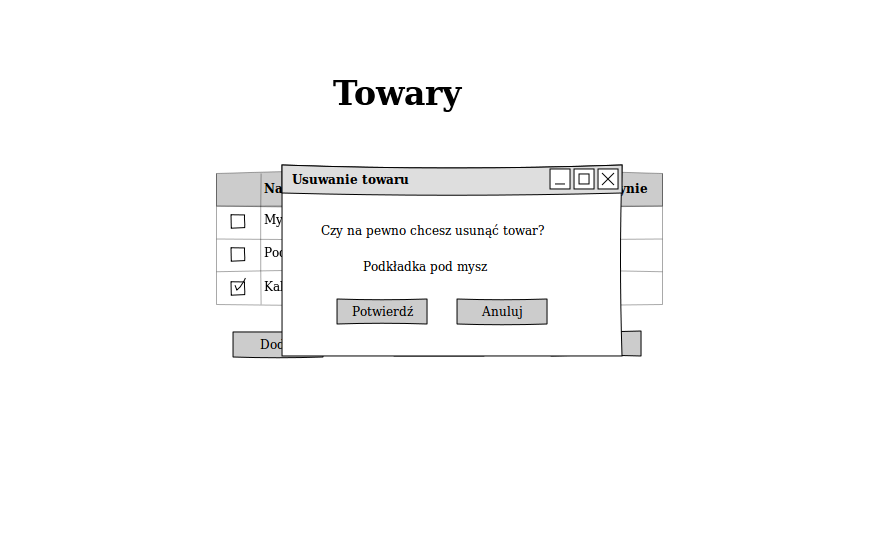
\includegraphics[scale=0.45]{../img/interfejs/usuniecie-danych-towaru.png}
  \end{center}
  \caption{Okno usunięcia danych towaru}
\end{figure}
\FloatBarrier

\begin{figure}[!htb]
  \begin{center}
    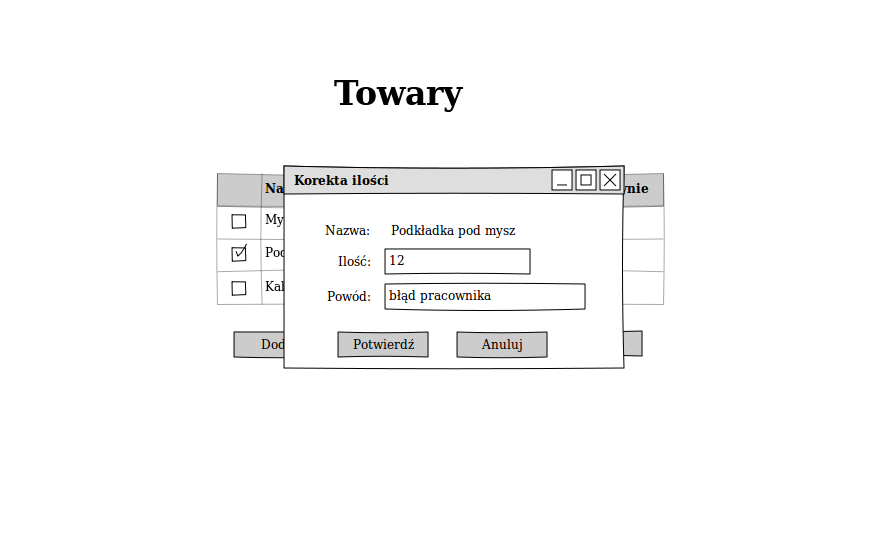
\includegraphics[scale=0.45]{../img/interfejs/korekta-ilosci-towaru.png}
  \end{center}
  \caption{Okno korekty stanu towaru}
\end{figure}
\FloatBarrier

\begin{figure}[!htb]
  \begin{center}
    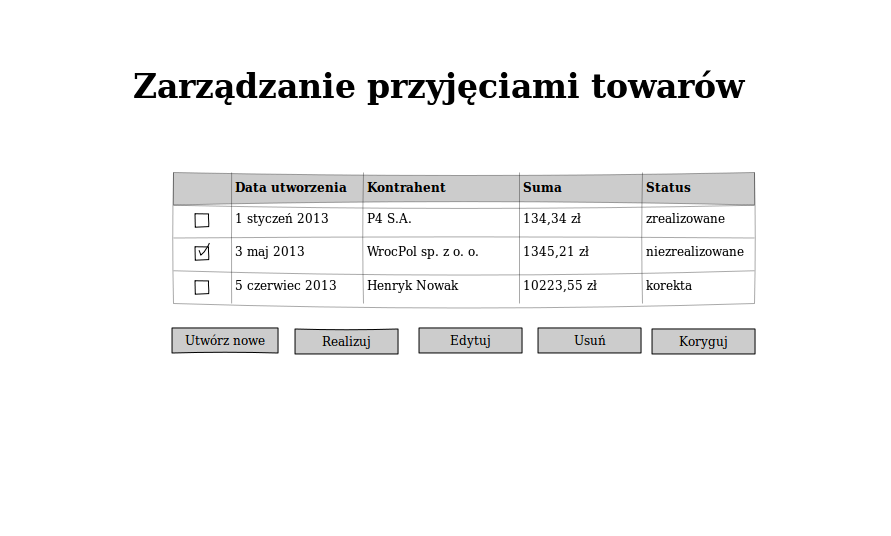
\includegraphics[scale=0.45]{../img/interfejs/zarzadzanie-przyjeciami-towaru.png}
  \end{center}
  \caption{Okno zarządzania przyjęciami towarów}
\end{figure}
\FloatBarrier

\begin{figure}[!htb]
  \begin{center}
    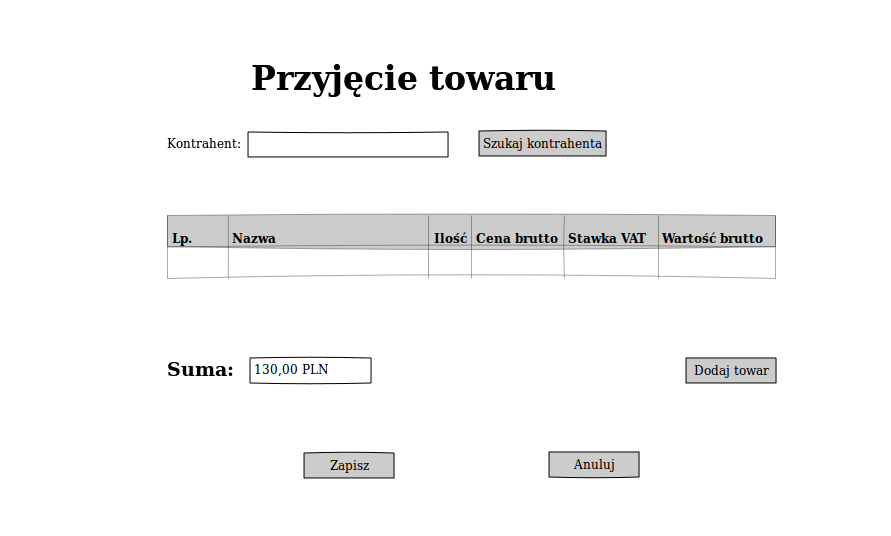
\includegraphics[scale=0.45]{../img/interfejs/utworzenie-przyjecia-towaru.png}
  \end{center}
  \caption{Okno utworzenie przyjęcia towaru}
\end{figure}
\FloatBarrier

\begin{figure}[!htb]
  \begin{center}
    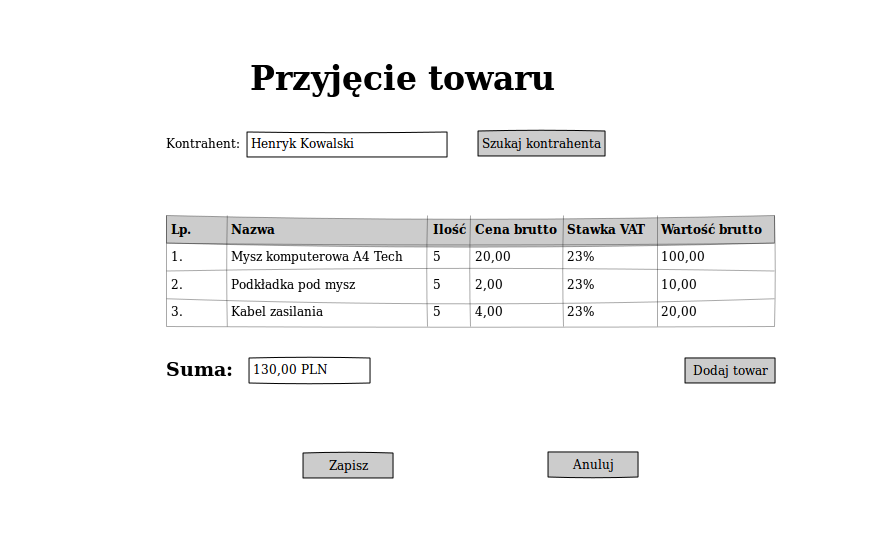
\includegraphics[scale=0.45]{../img/interfejs/edycja-przyjecia-towaru.png}
  \end{center}
  \caption{Okno edycji przyjęcia towaru}
\end{figure}
\FloatBarrier

\begin{figure}[!htb]
  \begin{center}
    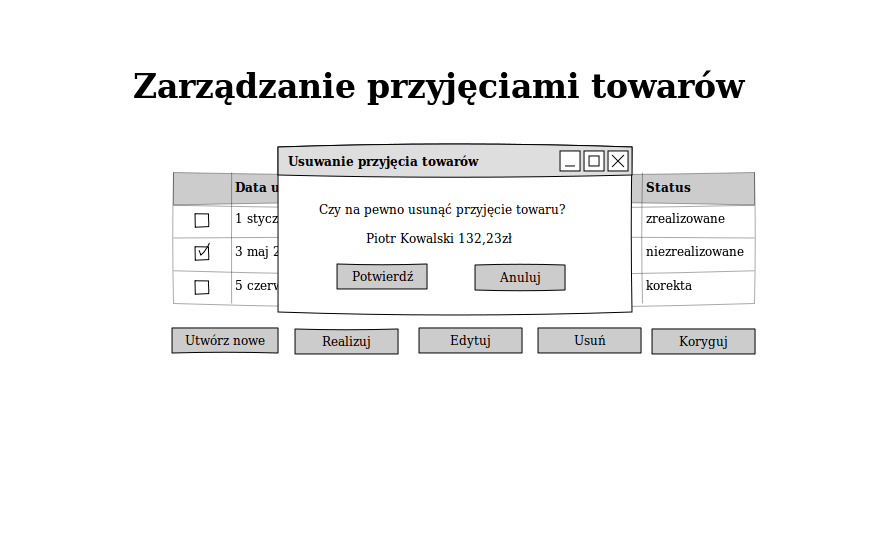
\includegraphics[scale=0.45]{../img/interfejs/usuniecie-przyjecia-towaru.png}
  \end{center}
  \caption{Okno usunięcia przyjęcia towaru}
\end{figure}
\FloatBarrier

\begin{figure}[!htb]
  \begin{center}
    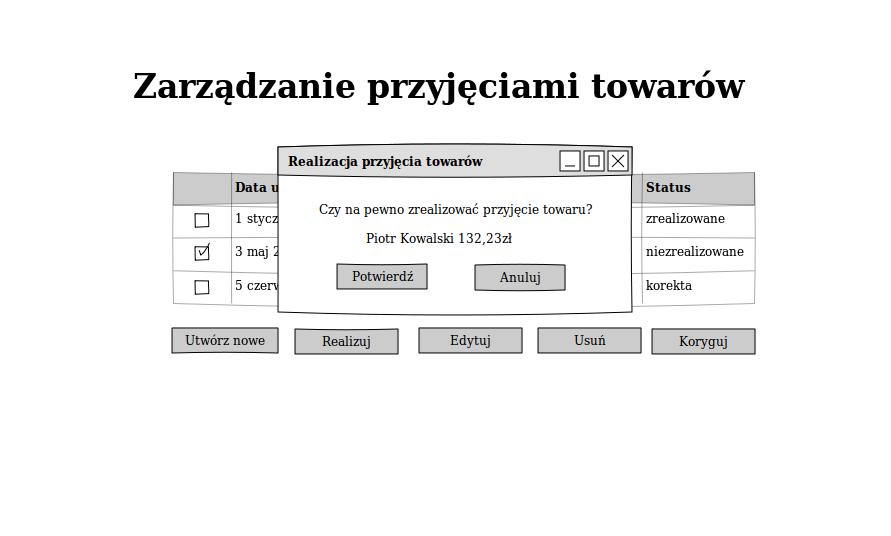
\includegraphics[scale=0.45]{../img/interfejs/realizacja-przyjecia-towaru.png}
  \end{center}
  \caption{Okno urealizacji przyjęcia towaru}
\end{figure}
\FloatBarrier

\begin{figure}[!htb]
  \begin{center}
    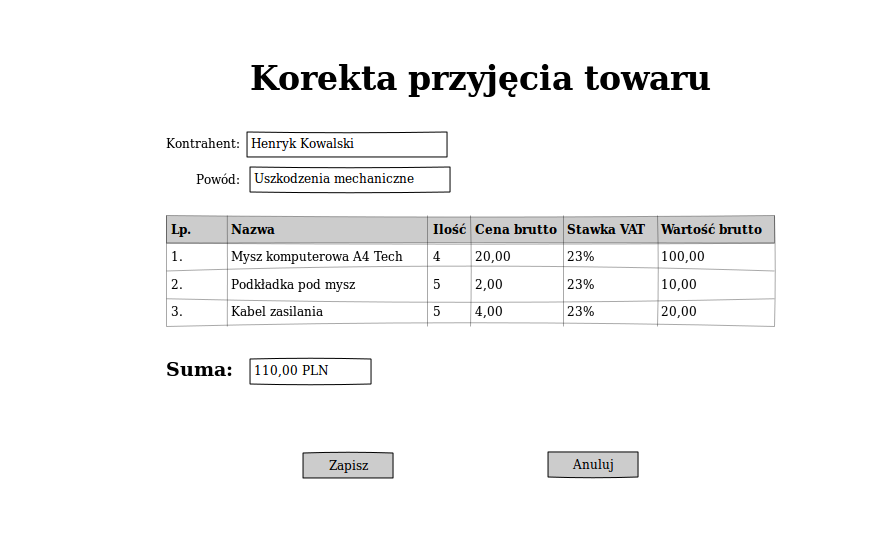
\includegraphics[scale=0.45]{../img/interfejs/korekta-przyjecia-towaru.png}
  \end{center}
  \caption{Okno korekty przyjęcia towaru}
\end{figure}
\FloatBarrier